\chapter{Experimental Analysis}
\section{Data Collection and Analysis}
The most important measurement to be made in order to perform significant analysis is the vibration signal. Improvements on this would be to collect some speed information and preferably some reference point on a turn of the shaft in the system. This is often performed using a once per turn reference mark on the shaft. Additionally, a spin speed measurement independent of the spin speed and with more time precision will aid in filtering and providing accuracy of frequency spectrum. An orthogonal vibration signal can help in characterizing non-symmetric systems, and allow for the visualization of the shaft centerline orbit path. For the correct characterization of the signals metioned thus far, it is important to also retain the sampling rates of the various signals.\par
There are two main figures that form the basis for other rotordynamic analysis techniques and figures. These are the Bode diagram and the Frequescy Spectrum. The Bode diagram plots the amplitude of vibration against speed alongside the phase angle  against speed. Frequency spectrum plots encapsulate frequency domain information gathered from the time domain amplitude data. A derivation of the Bode diagram, the Polar plot, plots the amplitude and phase of the signal as a vector on the polar plane as speed changes. Finally, the cascade plot cascades frequency spectrum plots as speed changes.\par
A difficulty in rotordynamic analysis arises in the change of speed of the system forcing much of the analysis to be performed in a short window in time. The window is typically made small enough to where the operation performed would be the same or similar if it had been performed on a stationary system. A generic ramping of speed, and inherently vibration, is depicted in Figure \ref{fig:PosOverTime}. The time domain signals will be represented as $ v(t)\ \&\ w(t) $ for an orthogonal set of transducers.\par 
\begin{figure}
	\centering
	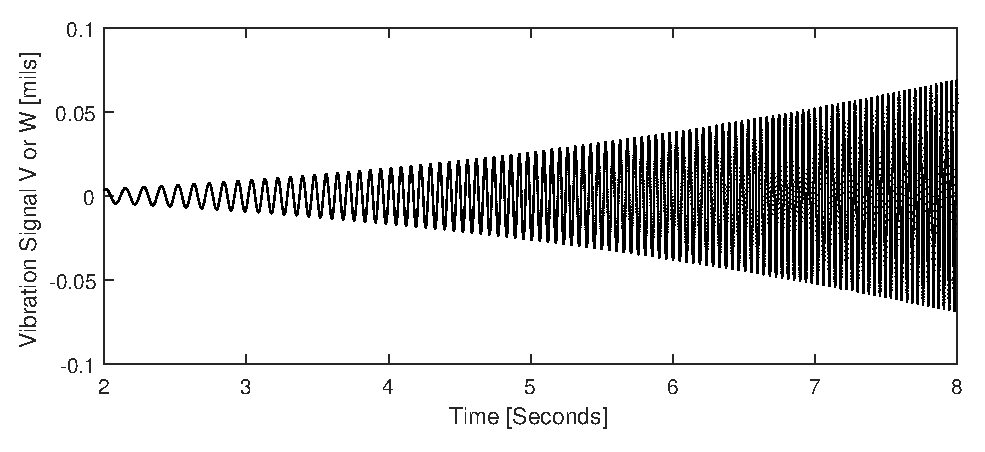
\includegraphics[width=\linewidth]{./figures/Pos_Over_Time.eps}
	\caption{Position of the rotor shaft over a certain timespan.}
	\label{fig:PosOverTime}
\end{figure}
To combat the dynamic nature of the system, a windowing approach is taken as depicted in figures \ref{fig:FreqSpanOverTime} and \ref{fig:FreqSpanWindow} Approaching the problem this way 
\begin{figure}
	\begin{subfigure}{.5\textwidth}
	\centering
	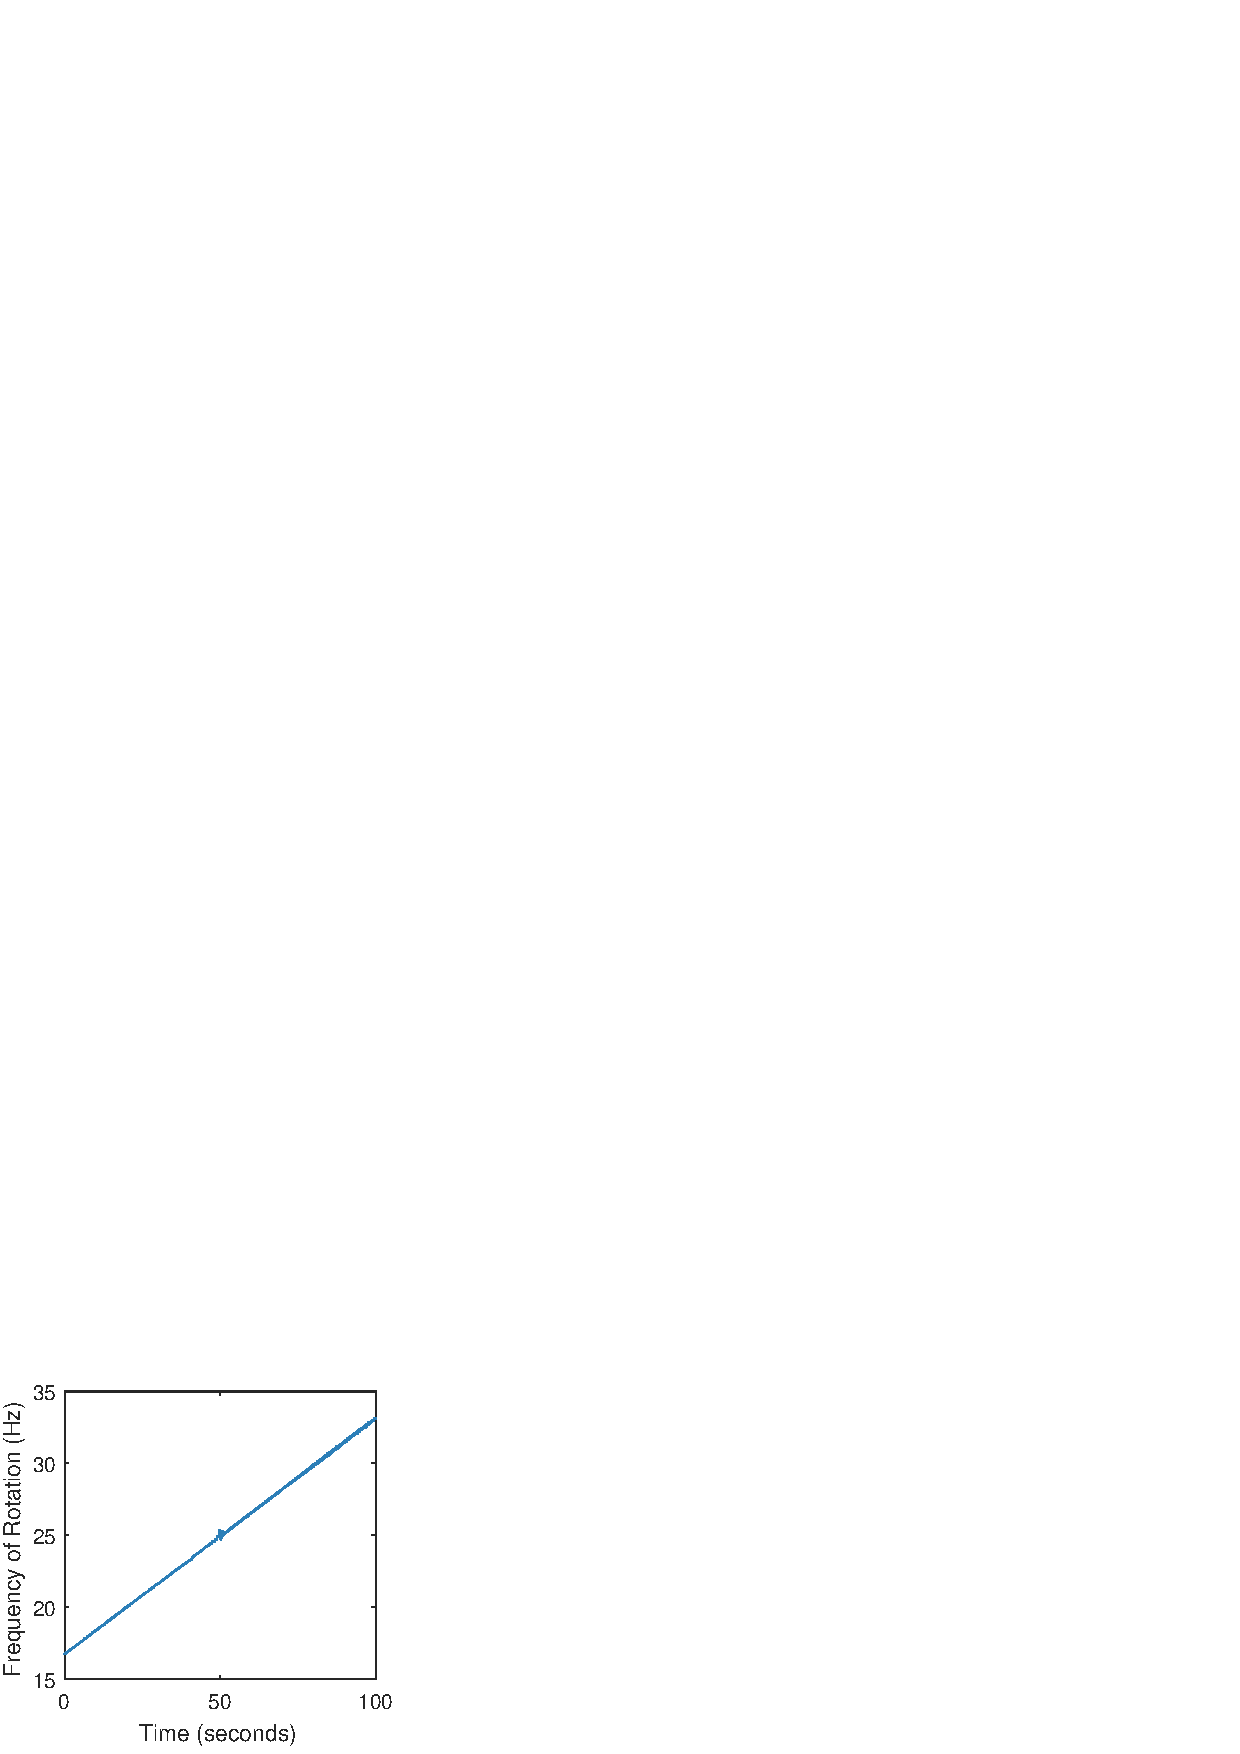
\includegraphics[width=\linewidth]{./figures/FrequencySpan.png}
	\caption{Rotor speed change over time during a ramp up.}
	\label{fig:FreqSpanOverTime}
\end{subfigure}
\begin{subfigure}{.5\textwidth}
	\centering
	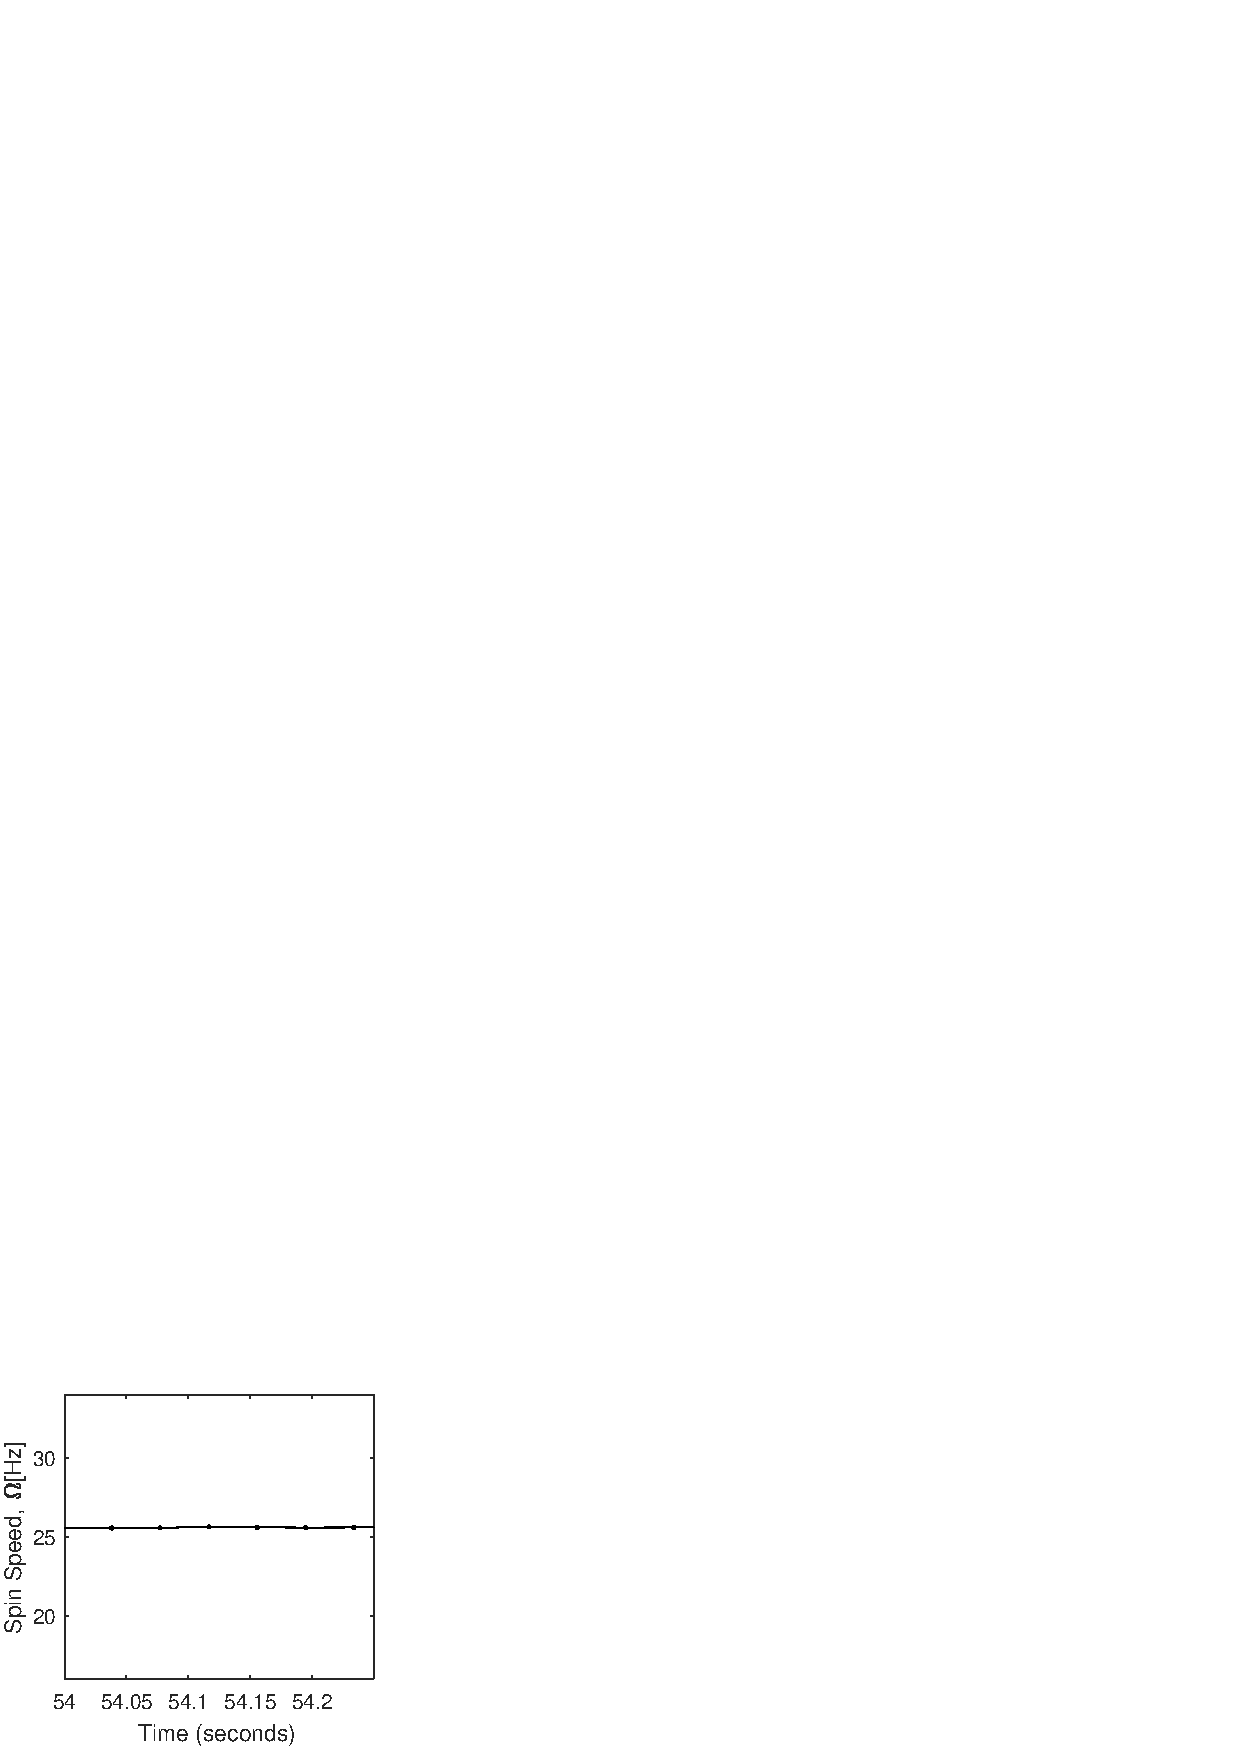
\includegraphics[width=\linewidth]{./figures/FrequencyWindow.png}
	\caption{Rotor speed change over time during a ramp up.}
	\label{fig:FreqSpanWindow}
\end{subfigure}
\end{figure}
Inside of a window of vibration, as the one shown in Figure \ref{fig:WindowedData}the Speed, Amplitude and Phase all approach constant the smaller the window gets.The Frequency Response has a twofold proportionality to window size; as the window gets smaller the frequency content of the signal itself approaches constant, but the resolution of the transform to approximate those frequencies decreases.\par
\begin{figure}
	\centering
	\includegraphics[width=\linewidth]{./figures/SteadyS.png}
	\caption{A window in time of the transient vibration signal in orthogonal directions.}
	\label{fig:WindowedData}
\end{figure}
The variables $ v(t) $ \& $ w(t) $ will now take the form $ v(n) $ \& $ w(n) $ inside the window in fig. \ref{fig:WindowedData}, where $ n $ is sample number. All of the plots to be presented here will be functions of two or more of the following variables: Amplitude[mils],Phase[Rad],Frequency Spectrum[mils], and Rotation Speed[RPM]. The Speed comes from the system so no analysis is necessary. Amplitude, Phase, and Frequency Spectrum must be calculated in windows of the data. Amplitude, Phase and speed are often combined into an array of vectors where speed is the index and Amplitude and Phase are the magnitude and angle of a vector, respectively.\par 
\subsection{Amplitude}
Amplitude calculation is fairly straightforward within the window of \ref{fig:WindowedData}. One approach to calculate the peak to peak vibration is to take the $ A_v = max(v)-min(v) $ over the whole sample, where $ A $ is the amplitude. Another is to use a peak-finding algorithm to determine the height of each peak and average them all over the sample length.
\subsection{Frequency Spectrum}
The frequency spectrum of the signal is calculated inside the window using the Fourier Transform. In MATLAB the Fast Fourier Transform has been preprogramed allowing easy working between time and frequency domains.
\begin{equation}\label{eq:FFTReal}
Y = \text{fft}(v),\ \&\ Z = \text{fft}(w)
\end{equation}
where X and Y must be scaled by the length of v and w to represent amplitude of vibration.\par 
A useful way to represent the data is using complex variable to compact the two orthogonal displacements $ v\ \&\ w $ as
\begin{equation}\label{eq:ComplexDisplacement}
z = v + iw
\end{equation}
now the frequency spectrum of this complex value represents both equations in one
\begin{equation}\label{eq:FFTComplex}
Z = \text{fft}(z)
\end{equation}
Thus far, the frequency spectrum in the real coordinates and in the complex is in terms of samples on the dependent axis. The frequency vector to which the fft() coresponds must be calculated. It is known that the slop of the frequency vector is $ df=Fs/N $, where Fs is the sampling rate of the time domain signals. It is also known that the frequency vector is the same length as the time domain signal 
\begin{equation*}
f=df(0:N-1)
\end{equation*}
but the spectrum needs to be centered at 0
\begin{equation*}
\begin{array}{c}
Q=(N+1)/2\\
f_Q=df(Q-1)\\
f_c=f-fQ
\end{array}
\end{equation*}
where $ f_c $ is the frequency vector that pairs with the real or complex frequency spectrum.
\subsection{Phase Angle}
\subsubsection{Time Domain Approach}
A rather direct way of calculating the phase angle comes from the interpretation of the time domain signal. If some once per turn reference is available, then using either a zero-crossing, peak-finding, or threshold algorithm can be employed to reference a specific angle of the shaft rotation. If the vibration signal is mostly synchronous, that is vibrating at the same frequency as the rotation of the shaft, then a peak-finding or zero-crossing algorithm can be used to determine the number of samples from the shaft reference angle to the peak of the vibration.\par 
\begin{equation}\label{eq:PhaseAngleTimeDomain}
\beta_i = 2\pi\frac{\#ref_i-\#peak_i}{\#ref_i-\#ref_{i-1}}
\end{equation}
where $ \beta_i $ is the phase lag of the signal of interest from the reference signal at the $ i $th reference cycle, $ \#ref_i $ is the sample number of the reference trigger, and $ \#peak_i $ is the sample number of the peak of the signal of interest. One large advantage to this brute force method is that is can run continuously and provide current phase information on just the last rotation of the shaft. In the application to the window of vibration data, fig. \ref{fig:WindowedData}, the measurements of each cycle would be averaged across the window to provide just one phase lag data point to match the one amplitude data point and the one speed data point.\par 
\subsubsection{Frequency Domain Approach}
Alternatively, the phase angle can be determined using the frequency domain signals.\par 
If the speed of the rotor is known and the time domain signals $ v\ \&\ w $ are known to be synchronous, or filtered to synchronous, then the spectrums of the signals of interest can be used to calculate the phase delay. calculate the fft of the time domain signal of interest and reference signals
\begin{equation*}
\begin{array}{c}
Y = \text{fft}(v)\\
K = \text{fft}(k)
\end{array}
\end{equation*}
where K and k are the freq. domain and time domain signals of the reference signal respectively. Now using the speed of synchronous vibration, find the bin that is a peak nearest to that speed. Calculate the angle of the complex number corresponding to that bin for both the reference and signal of interest
\begin{equation*}
\begin{array}{c}
\varphi_Y = atan2(Y(max_bin))\\
\varphi_K = atan2(K(max_bin))
\end{array}
\end{equation*} 
and finally, the phase delay $ \beta_y=\varphi_K-\varphi_Y $
\section{Experimental Plots}\label{ExperimentalPlots}
In the previous section Amplitude, Phase, and frequency spectrum were calculated for the interior of a window on the data as a whole. Each of the data then need to be indexed on the speed for that window and continue until the entire signal has been exhausted. The Bode, and the Cascade plots can now be formed.\par 
for the visualization of the plots, experimental data from a overhung rotor system with one disk will used to calculate the figures.\par
\subsection{Bode}
The Bode diagram is the stacked plot containing amplitude as a function of speed on top of phase as a function of speed. A Bode plot for the system mentioned in the \S\ref{ExperimentalPlots} is given in Figure \ref{fig:ExpExampleBode}. Notice how the Vertical plane undergoes a critical speed before the horizontal plane. This is an indication of high anisotropy of stiffness in the system. By observing the phase lag of each the vertical and the horizontal, it is evident that the orbit direction is opposite the spin speed between speeds ~ 1280-1350[RPM]. This is due to the phase angles switching polarity with one another. If normally horizontal lags vertical, as is suggested by the sub-synchronous and super-synchronous range, then during the critical speed the orbit is reversed since vertical begins to lag horizontal.
\begin{figure}
	\def\width{\linewidth/1.5}
	\def\height{\linewidth/3}
	\def\sep{3em}
	\pgfplotsset{every picture/.style={scale=1},every axis/.style={title style={yshift=-.8em}}}%, every axis/.style={hide axis}}%
	\centering
	\import{figures/}{ExpExampleBode.tex}
	\caption{Bode diagram of the experimental system described in \S\ref{ExperimentalPlots}. Red is horizontal plane, and blue is vertical.}
	\label{fig:ExpExampleBode}
\end{figure}
\subsection{Cascade}
The Cascade plot is a cascade, or waterfall of the spectrum at either various spin speeds, or in the case of the waterfall plot, at various times. A Cascade plot is demonstrated with the experimental system described in \S\ref{ExperimentalPlots}, as Figure \ref{fig:ExpExampleCascade}. Now using this figure it is easy to detect the portion of the start-up in which the orbit is opposite the spin speed. A sharp dip in positive resonances correlated with a sharp rise in negative ones leads to this phenomena caused by the anisotropy in the stiffness matrix.\par 
The Cascade plot is particularly useful in characterizing non-synchronous vibration. Slightly evident in the example cascade of figure \ref{fig:ExpExampleCascade} is the super-synchronous vibration at twice the spin speed, this is often called the 2X vibration and likewise and other non-synchronous whirl can be referenced as nX. The cascade plot is an indispensable tool for the analysis of fluid film bearing as they are characterized by sub-synchronous whirl that is difficult to identify in a Bode Diagram.\par 
\begin{figure}
	\centering
	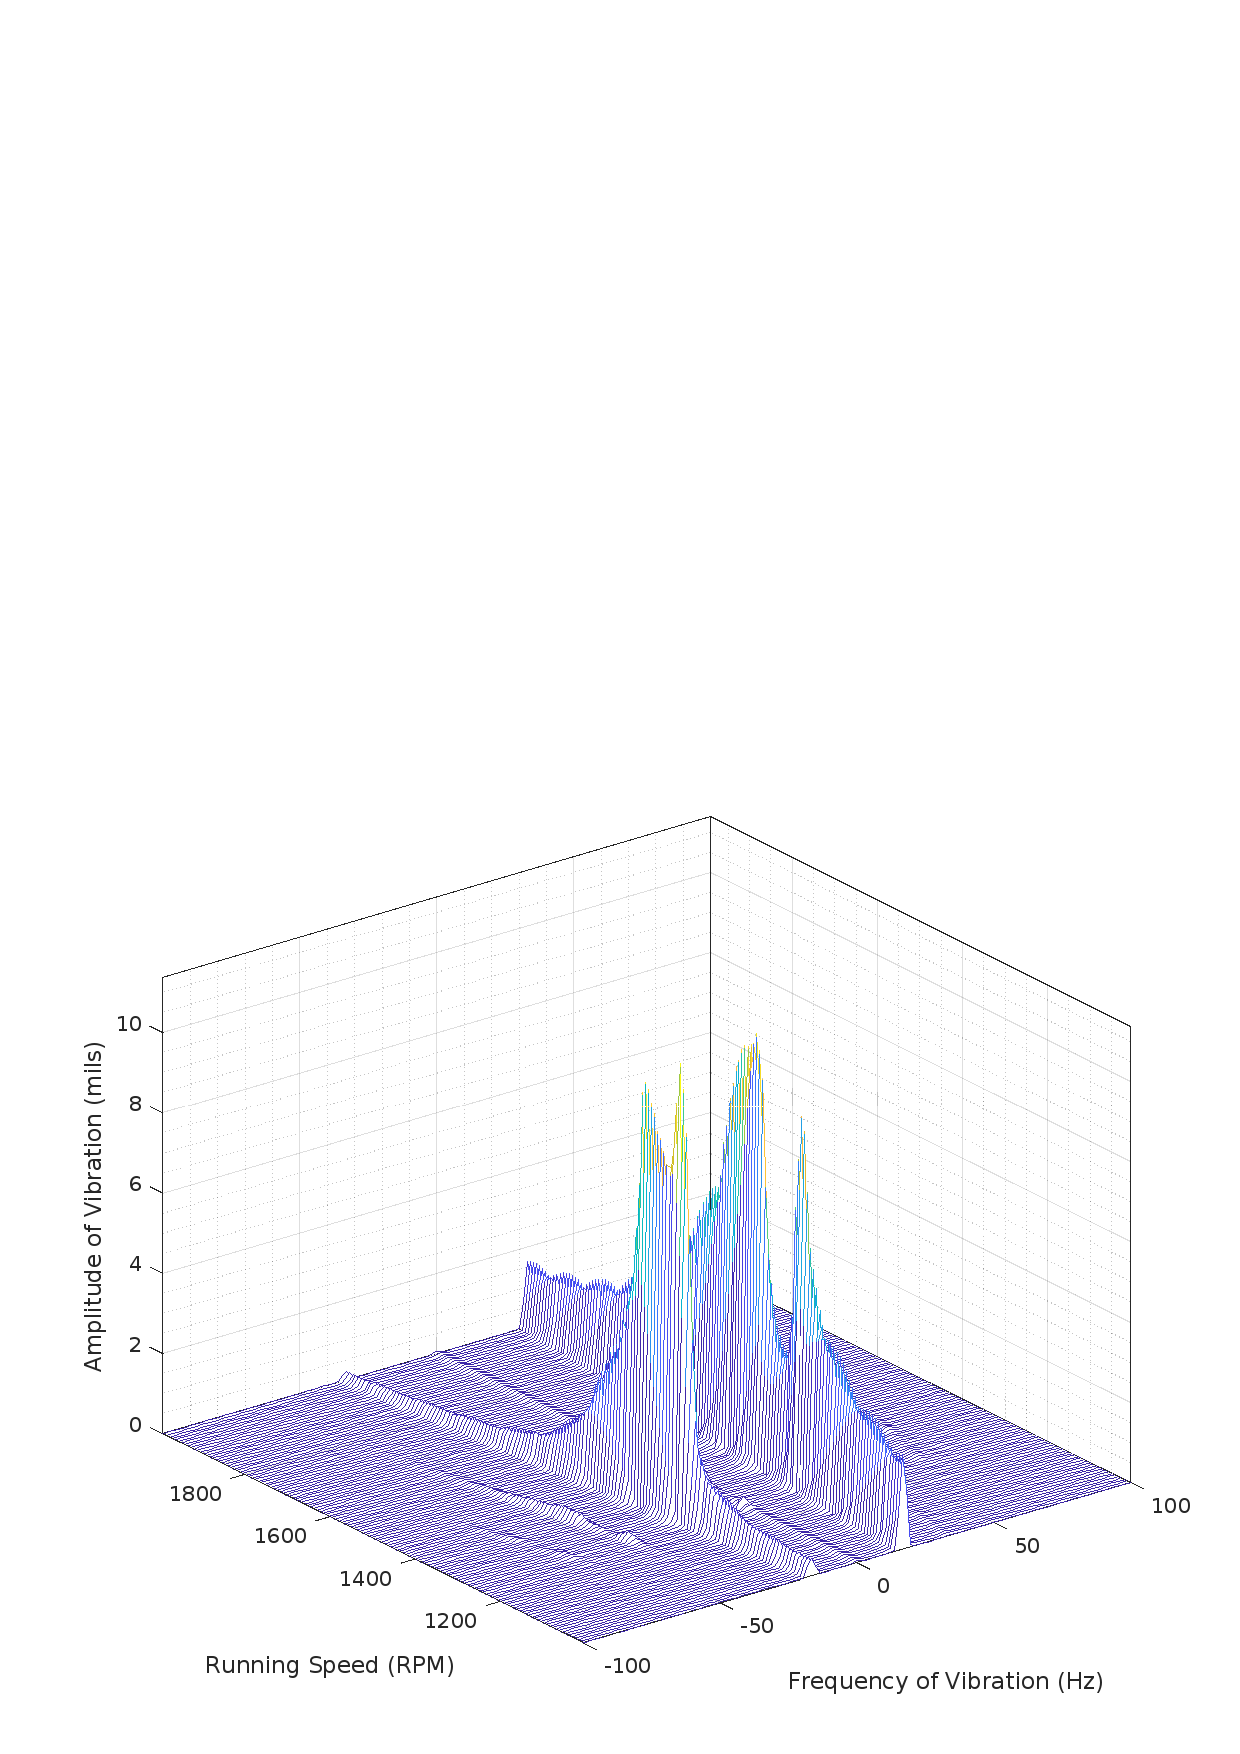
\includegraphics[width=\linewidth]{./figures/ExpExampleCascade.pdf}
	\caption{Cascade of the experimental system described in \S\ref{ExperimentalPlots}.}
	\label{fig:ExpExampleCascade}
\end{figure}
\subsection{Orbit}
Now in the ``real'' space, the actual orbit or trace of the centerline of the shaft is observed. In this work, the orbit is visualized in two ways; as a path in 2D space at a specific spin speed, or as a 3D orbit with a cascade of orbits as spin speed is increased. The 3D Orbit allows for the visualization of complex phenomena in a unique physical way where the shapes feel more real. Figure \ref{fig:ExpExample3DOrbit} 3D Orbit is given for the experimental example described in \S\ref{ExperimentalPlots}. Appearing, once again is evidence of the negative whirl in the critical speed range. In the 3D orbit a necking of the shape can be seen between the speeds of 1200-1400[RPM] indicating the orbit has reversed its direction. Looking at independent orbits at specific speeds should explicitly demonstrate the orbit necking and turning negative.\par
\begin{figure}
	\centering
	\includegraphics[width=\linewidth]{./figures/ExpExample3DOrbit.pdf}
	\caption{3DOrbit of the experimental system described in \S\ref{ExperimentalPlots}.}
	\label{fig:ExpExample3DOrbit}
\end{figure}
\begin{figure}
\begin{subfigure}{.25\linewidth}
	\def\width{\linewidth}
	\pgfplotsset{every picture/.style={scale=1},every axis/.style={title style={yshift=-.8em}}}%, every axis/.style={hide axis}}%
	\centering
	\import{figures/}{ExpExampleOrbit1194.tex}
	\label{fig:ExpExampleOrbit1194}
\end{subfigure}
\begin{subfigure}{.25\linewidth}
	\def\width{\linewidth}
	\pgfplotsset{every picture/.style={scale=1},every axis/.style={title style={yshift=-.8em}}}%, every axis/.style={hide axis}}%
	\centering
	\import{figures/}{ExpExampleOrbit1203.tex}
	\label{fig:ExpExampleOrbit1203}
\end{subfigure}
\begin{subfigure}{.25\linewidth}
	\def\width{\linewidth}
	\pgfplotsset{every picture/.style={scale=1},every axis/.style={title style={yshift=-.8em}}}%, every axis/.style={hide axis}}%
	\centering
	\import{figures/}{ExpExampleOrbit1206.tex}
	\label{fig:ExpExampleOrbit1206}
\end{subfigure}
\begin{subfigure}{.5\linewidth}
	\def\width{.45\linewidth}
	\pgfplotsset{every picture/.style={scale=1},every axis/.style={title style={yshift=-.8em}}}%, every axis/.style={hide axis}}%
	\centering
	\import{figures/}{ExpExampleOrbit1222.tex}
	\label{fig:ExpExampleOrbit1222}
\end{subfigure}
\begin{subfigure}{.5\linewidth}
	\def\width{.5\linewidth}
	\pgfplotsset{every picture/.style={scale=1},every axis/.style={title style={yshift=-.8em}}}%, every axis/.style={hide axis}}%
	\centering
	\import{figures/}{ExpExampleOrbit1289.tex}
	\label{fig:ExpExampleOrbit1289}
\end{subfigure}
\caption{Orbits of the experimental example. Spin speed is counterclockwise.}\label{fig:ExpExampleOrbits}
\end{figure}
Inspection of the orbits of Figure \ref{fig:ExpExampleOrbits} reveals that the orbit is whirling backward between the speeds 1205-1280[RPM].
\subsection{Filtering}
Correlating phase angles between real signals can be extremely difficult due to the noise and harmonic frequencies that may disrupt the measurement. Furthermore, it can be useful to decompose a real signal into specific harmonic components of the spin speed. One such instance is in the analysis of a fluid film bearing. Often the fluid film bearing will cause an unbalance at the subsynchronous frequency of just under 0.5X. Using a filter, the response of the system to this specific frequency can be extracted, allowing the analysis of phase angle and amplitude directly due to the influence of interest.\par 
MATLAB has an extensive library of digital filters that can be adjusted to filter specific frequency ranges with no phase delay, and recall the states from the previous window as to not loose dynamic information from one step to the next.\par 
A synchronous filter was applied the experimental example and the cascade plot is shown in Figure \ref{fig:ExpExampleCascade2}. All amplitudes of frequencies other than the synchronous frequencies have been eliminated. This system did not have strong super- or sub-synchronous response, so this filtering does not make an appreciable effect to the Bode plot. But, with many real systems filtering will be necessary to analyze the system.
\begin{figure}
	\centering
	\includegraphics[width=\linewidth]{./figures/ExpExampleCascade2.pdf}
	\caption{Cascade of the experimental system witha synchronous filter applied.}
	\label{fig:ExpExampleCascade2}
\end{figure}